%!TEX encoding = UTF8
%!TEX root =notes.tex

\section{Fonctions affines}

\subsection{Définitions}

La notion de fonctions affines généralise celle de suite arithmétique.
Un suite est définie comme une fonction associant à tout entier naturel $n\in\N$ un nombre réel.
Un fonction affine, quant à elle, n'a pas cette restriction : elle peut prendre n'importe quel nombre réel comme antécédant, et une image lui sera associé.

\dfn{Fonction affine}{
	Un \emph{fonction affine} est une fonction $f$ associant à tout réel $x\in\R$ un réel $f(x)\in\R$ tel que
		\[ f(x) = ax + b, \]
	où $a$ et $b$ sont deux paramètres : le coefficient directeur et l'ordonnée à l'origine.
}{}


\exe{}{
	On considère une suite arithmétique $u$ telle que
		\[ u(0) = 3, \qquad\text{ et }\qquad u(1) = 8.\]
	Le chapitre $1$ nous permet de donner le terme de rang $n\in\N$ pour tout $n$ de la suite.
	En effet, son terme initial est $3$, et sa raison est donnée par
		\[ u(1) - u(0) = 8-3 = 5. \]
	Ainsi, le théorème \ref{thm:lili} implique que
		\[ u(n) = 5n + 3, \]
	pour tout $n\in\N$.
	
	Considérons désormais une fonction affine $f$ telle que
		\[ f(0) = 3, \qquad \text{ et } \qquad f(1) = 8. \]
	Comme $f(x) = ax+b$ pour tout $x\in\R$ et pour certains paramètres $a,b\in\R$, les données ci-dessus sont équivalentes à
		\[ a \times 0 + b = 3 \qquad \text{ et } \qquad a\times1 + b = 8. \]
	Par suite, $b=3$, et $a= 8-b = 8-3 = 5$. Par conséquent,
		\[ f(x) = 5x + 3 \qquad \text{ pour tout } x\in\R. \]
}{}

\nt{
	Comme pour les suites arithmétiques, les fonctions affines vérifient
		\[ f(x+1) - f(x) = a(x+1) + b - (ax + b) = a, \]
	pour n'importe quel $x\in\R$ (et donc en particulier pour $x\in\N$ entier naturel, comme dans l'équation \eqref{eq:1}).

}

\dfn{Repère et point}{
	On définit le plan, espace en deux dimension, par un ensemble de couples $(x,y)$ où $x,y\in\R$ sont deux réels.
	En d'autres termes, c'est l'ensemble
		\[ \{(x,y) \text{ tq. } x \in\R, \text{ et } y \in \R \} \]
	
	On appelle chaque couple un \emph{point} du plan, et ses coordonnées son \emph{abscisse} et son \emph{ordonnée}.
}{}

\ex{}{
	\begin{multicols}{2}
		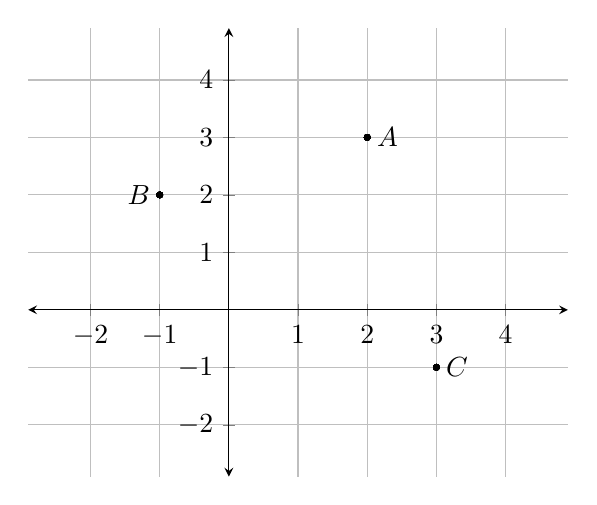
\begin{tikzpicture}[>=stealth, scale=1]
		\begin{axis}[xmin = -2.9, xmax=4.9, xtick={ -3, ..., 5}, ymin=-2.9, ymax=4.9, ytick={-3, ..., 5}, axis x line=middle, axis y line=middle, axis line style=<->, xlabel={}, ylabel={}, grid=both]
			
			\addplot[black, mark=*, mark size = 1] (2,3) node[above, right] {$A$};
			\addplot[black, mark=*, mark size = 1] (-1,2) node[above, left] {$B$};
			\addplot[black, mark=*, mark size = 1] (3,-1) node[below, right] {$C$};
		\end{axis}
	\end{tikzpicture}
	
	Les points $A$, $B$, et $C$ admettent pour coordonnées
		\begin{align*}
			A(2;3), && B(-1;2), && C(3;-1).
		\end{align*} 
	\end{multicols}
}{}

\nt{
	En mathématiques, on définit un ensemble de la façon suivante :
		\[ \{ \text{élément} \in \text{ensemble} \text{ tq. } \text{condition vérifiée} \}. \]
	L'ensemble ainsi décrit désigne tous les éléments appartenant à l'ensemble vérifiant la condition.
}

\exe{}{
	Décrire les ensembles suivants :
		\begin{multicols}{2}
		\begin{enumerate}
			\item $\{ x \in \R \text{ tq. } x \geq 2\}$
			\item $\{ x \in \R \text{ tq. } x \neq 0\}$
			\item $\{ n \text{ tq. } n\in\N \text{ ou } -n \in \N \}$
			\item $\left\{ \dfrac{a}{b} \text{ tq. } a,b\in\Z \text{ et } b\neq 0\right\}$
		\end{enumerate}
		\end{multicols}
}{}

\dfn{Droite du plan}{
	Une \emph{droite} est un ensemble de points du plan.
	Ce sont tous les points qui vérifient une condition affine :
		\[ \{ (x,y) \text{ tq. } x,y\in\R, \text{ et } y = ax+b \}, \]
	où $a,b\in\R$ sont des paramètres qui définissent entièrement la droite.
}{def:droite}

\ex{}{
	La droite $(d)$ donnée par
		\[ (d) = \{ (x,y) \text{ tq. } x,y\in\R \text{ et } y = x \} \]
	correspond à l'ensemble des points du plan dont l'abscisse est égale à l'ordonnée.
	
	Ainsi, $(3;3) \in (d)$ et $(-\sqrt{2}; -\sqrt{2}) \in (d)$, mais $(3;4) \notin (d)$.
	On peut facilement dessiner la droite à partir de deux points.
	
		\begin{center}
		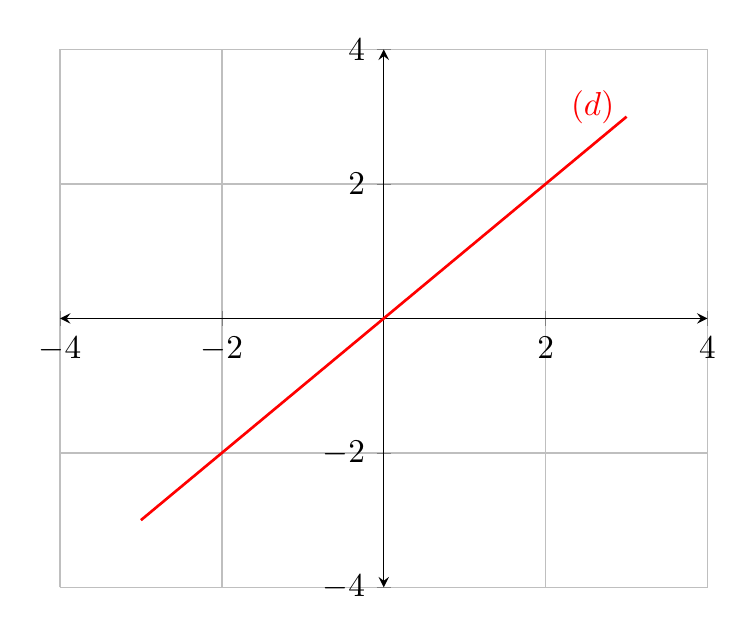
\begin{tikzpicture}[>=stealth, scale=1.2]
		\begin{axis}[xmin = -4, xmax=4, ymin=-4, ymax=4, axis x line=middle, axis y line=middle, axis line style=<->, xlabel={}, ylabel={}, grid=both]
		
			\addplot[red, thick, domain =-3:3, samples=2] {x}  node[above=3pt, left] {$(d)$};
		
			
		\end{axis}
	\end{tikzpicture}
	\end{center}

}{}


\ex{}{
	La droite $(d)$ donnée par
		\[ (d) = \{ (x,y) \text{ tq. } x,y\in\R \text{ et } y = x+6 \} \]
	correspond à l'ensemble des points du plan dont l'ordonnée est égale à l'abscisse plus $6$.
	
	Ainsi, $(3;9) \in (d)$ et $(-\sqrt{2}; -\sqrt{2}+6) \in (d)$, mais $(6;0) \notin (d)$.
	On peut facilement dessiner la droite à partir de deux points.
	
		\begin{center}
		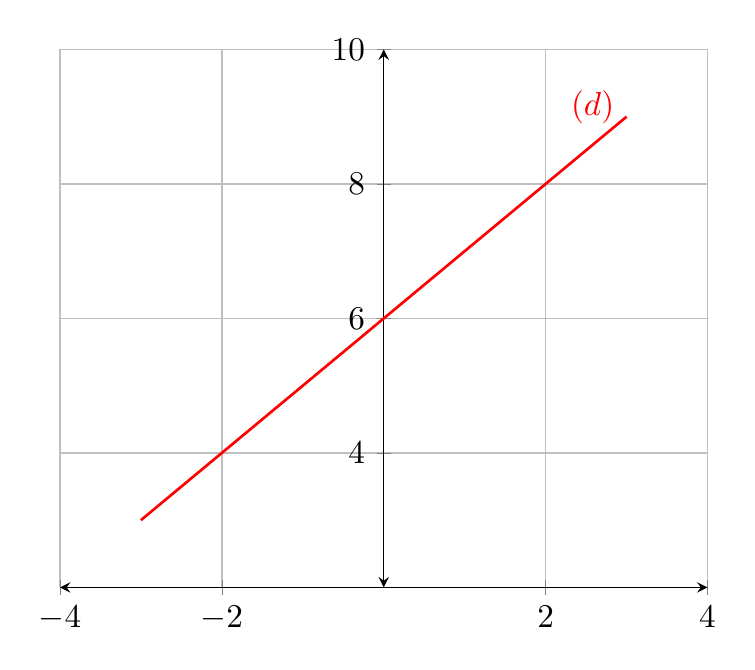
\begin{tikzpicture}[>=stealth, scale=1.2]
		\begin{axis}[xmin = -4, xmax=4, ymin=2, ymax=10, axis x line=middle, axis y line=middle, axis line style=<->, xlabel={}, ylabel={}, grid=both]
		
			\addplot[red, thick, domain =-3:3, samples=2] {x+6}  node[above=3pt, left] {$(d)$};
		
			
		\end{axis}
	\end{tikzpicture}
	\end{center}

}{ex:droite}

\nt{
	À partir de la représentation de la droite de l'exemple \ref{ex:droite}, on peut extraire deux points, $(0;6)$ et $(1,7)$ et appliquer la lecture graphique en tant que suite arithmétique.
	 Le terme initial est $6$ et la raison $1$, ce qui donne $u(n) = n + 6$ pour tout $n\in\N$, à comparer avec la fonction $f(x) = x+6$ pour tout $x\in\R$.
}

\ex{}{
	Donner deux points distincts appartenant à la droite suivante.
		\[ (d) = \{ (x,y) \text{ tq. } x,y\in\R \text{ et } y = 2x-1 \}. \]
	Représenter la droite dans un repère.
}{}

\subsection{Conséquences importantes}

\nt{
	À chaque droite $(d)$ est ainsi associée une fonction affine $f$ de telle sorte que
		\[ (d) = \{ (x,y) \text{ tq. } x,y\in\R \text{ et } y = f(x) = ax+b \}, \]
	pour certains paramètres $a,b\in\R$.
}


\thm{Propriété fondamentale}{
	Soit $(d)$ une droite et $f$ sa fonction affine associée.
		
	Un point $(x,y)$ appartient à la droite $(d)$ si et seulement s'il vérifie la condition de l'ensemble $(d)$.
	C'est-à-dire
		\[ (x,y) \in (d) \qquad\iff\qquad y = f(x). \]
}{thm:prop-fond}


\nt{
	Soit $(d)$ une droite et $f$ sa fonction affine associée :
		\[ f(x) = ax+b \qquad\text{ pour tout }x\in\R, \]
	pour certains paramètres $a,b\in\R$.
	
	Lorsque $x=0$, on a $f(0) = a\times0 + b = b$.
	Ainsi, d'après la propriété fondamentale, le point $(0 ; b)$ appartient à la droite $(d)$.
	C'est en fait le seul point de la droite à abscisse nulle. 
	
	Le paramètre $b$ est par conséquent l'ordonnée du point d'abscisse nulle ou, autrement dit, l'\emph{ordonnée à l'origine} de l'axe des abscisse.
}

\ex{}{
	Soient $(1;2)$ et $(4;-4)$ deux points du plan qui appartiennent à une droite appelée $(d)$.
	Notons $a,b \in\R$ les paramètres définissant la droite : 
		\[ (d) = \{ (x,y) \text{ tq. } x,y\in\R \text{ et } y = ax+b \}.\]
	On a les équivalences suivantes
		\[ (1;2) \in (d) \qquad\iff\qquad 2 = a\times1 + b, \]
	et
		\[ (4;-4) \in (d) \qquad\iff\qquad -4 = a\times4 + b. \]
	Ces deux égalités étant valides simultanément, on les met dans un système :
		\[ \begin{cases*} a + b = 2, \\ 4a + b = -4. \end{cases*} \]
	On souhaite isoler une inconnue afin de la déterminer.
	On peut alors soustraire la deuxième équation à la première de telle sorte que
		\begin{align*}
			(4a + b) - (a+b) &= (-4) - (2) \\
			4a+b-a-b & = -6 \\
			3a &= -6 \\
			a &= -2
		\end{align*}
	On remplace la valeur de $a$ dans une des deux équations du système pour trouver $b$ : $b=2-a = 4$.
	
	On conclut donc que la droite $(d)$ est donnée par
		\[ (d) = \{ (x,y) \text{ tq. } x,y\in\R \text{ et } y = -2x+4 \}.\]
}{ex:systeme-affine}

\exe{}{
	Vérifier que les points $(1;2)$ et $(4;-4)$ appartiennent bien à la droite 
		\[ (d) = \{ (x,y) \text{ tq. } x,y\in\R \text{ et } y = -2x+4 \}.\]
}{}

\mprop{}{
	Une droite est déterminée entièrement par l'appartenance de deux points distincts.
}{}

\nt{
	Il n'est pas surprenant qu'en géométrie, une droite soit donnée par deux points.
	Cependant, nous étudions ici la définition algébrique d'une droite : c'est un ensemble de points vérifiants une certaine équation affine.
	Il n'est pas clair \emph{a priori} que deux éléments d'un ensemble infini suffisent à déterminer tout cet ensemble.
	
	Remarquons cependant qu'une droite est déterminée entièrement par la valeur des deux paramètres $a$ et $b$ de la définition \ref{def:droite}.
	Or, deux équations distinctes suffisent à déterminer la solution d'un système linéaire à deux inconnues.
	
	Ceci se généralise sans peine. Par exemple, pour trouver une parabole de la forme $f(x)=ax^2 + bx + c$, il suffit de trois informations distinctes.
}

\exe{}{
	Décrire entièrement la droite $(d)$ contenant les points $(3;-4)$ et $(-2;14)$.
}{}

\exe{Approfondissement}{
	Décrire l'ensemble
		\[ (P) = \{ (x,y) \text{ tq. } x,y\in\R \text{ et } y=ax^2 + bx + c \} \]
	contenant les points $(0;1), (1;0),$ et $(2;1)$.
	Grapher la parabole, par exemple en écrivant \texttt{y=x² -2x + 1} sur \href{https://www.geogebra.org/calculator}{https://www.geogebra.org/calculator}.
}{}

\str{
	La stratégie de l'exemple \ref{ex:systeme-affine} peut se généraliser.
	Considérons $(x_A, y_A)$ et $(x_B, y_B)$ deux points distincts appartenant à une droite 
		\[ (d) = \{ (x,y) \text{ tq. } x,y\in\R \text{ et } y = ax+b \},\]
	où $a,b\in\R$ sont deux paramètres à déterminer.
	
	Les deux appartenances donnent les égalités suivantes, grâce au théorème \ref{thm:prop-fond}.
		\[ \begin{cases} y_A = ax_A + b, \\ y_B = ax_B + b. \end{cases} \]
	On rappelle ici que $(x_A,y_A)$ et $(x_B,y_B)$ sont des valeurs sues, et qu'il faut déterminer $a$ et $b$ en fonction de ces valeurs.
	
	On soustrait la deuxième équation à la première pour éliminer la variable $b$ et obtenir
	\begin{align*}
		y_A - y_B &= (ax_A + b) - (ax_B + b) \\
		y_A - y_B & = a(x_A - x_B) \\
		a & = \dfrac{y_A - y_B}{x_A - x_B}
	\end{align*}
	On peut ensuite substituer pour exprimer $b$ en fonction en fonctions des valeurs sues, mais la formule est moins facile à retenir.
		\[ b = y_A - \dfrac{y_A - y_B}{x_A - x_B} x_A = \dfrac{x_A y_B - x_B y_A}{x_A-x_B}. \]
}


\thm{}{
	Soit $(d)$ une droite donnée par	
		\[ (d) = \{ (x,y) \text{ tq. } x,y\in\R \text{ et } y = ax+b \}, \]
	pour certains paramètres $a,b\in\R$.
	
	Si $(x_A, y_A)$ et $(x_B, y_B)$ sont distincts et appartiennent à $(d)$, alors
		\begin{align*}
			a = \dfrac{y_A - y_B}{x_A - x_B} && \text{et} && b = \dfrac{x_A y_B - x_B y_A}{x_A-x_B}. 
		\end{align*}
}{thm:param-affine}


\exe{}{
	Calculer $a$ et $b$ de l'exemple \ref{ex:systeme-affine} à l'aide des formules ci-dessus et comparer avec les valeurs obtenues.
}{}
\exe{}{
	Décrire entièrement la droite contenant les points $(-1;-10)$ et $(1;30)$.
}{}


\nt{
	Considérons une droite $(d)$ associée à une fonction affine $f(x) = ax+b$, $x\in\R$.
	Le théorème \ref{thm:param-affine} dit que, pour $x_1, x_2 \in\R$ deux réels distincts,
		\[ a = \dfrac{f(x_1) - f(x_2)}{x_1 - x_2}. \]
	Remarquons que, si on pose $x_2 = n \in \N$ un entier naturel, et $x_1 = n+1$, on retrouve
		\[ a = f(n+1) - f(n), \]
	non sans rappeler la définition de la raison d'une suite (voir \eqref{eq:1}).
	
	L'importance du théorème est que les réels $x_1$ et $x_2$ ne sont pas nécessairement entiers, et pas nécessairement à distance $1$ l'un de l'autre.
}

\subsection{Lecture graphique}



\subsection{Parallélisme et intersection}
